\documentclass[11pt,a4paper]{article}
\usepackage{amsmath}
\usepackage{natbib}
\usepackage[margin=1in]{geometry}
\usepackage{setspace}
\usepackage{graphicx}
\usepackage{booktabs}

\setstretch{1.5}


\title{On the hierarchical structure: factor, accuracy and construction}
\author{Bohan Zhang}

\begin{document}

\maketitle

\section{Simulation}

To better control the factors such as trend, seasonality, dependence, we assume the bottom-level series are generated by the following innovative state space model:
\[
    \begin{aligned}
        y_t &= l_{t-1} + b_{t-1} + s_{t-m} + \varepsilon_t \\    
        l_t &= l_{t-1} + b_{t-1} + \alpha\varepsilon_t \\
        b_t &= b_{t-1} + \beta \varepsilon_t \\
        s_t &= s_{t-m} + \gamma\varepsilon_t,
    \end{aligned}
\]
where $l_t, b_t, s_t$ are level, trend and seasonal states. $\varepsilon_t$, called innovation, is the error term. 
$\alpha, \beta, \gamma$ are smoothing parameters which controls the pattern of the simulated time series. 
$m$ is the seasonal period.
This model is also known as ExponenTial Smoothing model with additive trend, additive seasonality and additive error, i.e., ETS(A, A, A)(\Citealp{ForecastingExponentialSmoothing}). 

\subsection{Scenario 1: Groups of time series sharing similar pattern}
We start from a simple hierarchy with one total node and four children nodes.
These four time series are expected to belong to two groups having different patterns, but two time series within the same group shares similar patterns. 
We control the ``similar'' pattern through the smoothing parameters, innovation term and seasonal spikes.

In this scenario, $m$ is set to $12$. The initial states $l_0, b_0, s_0, \dots, s_{1-m}$ are simulated from $\mathcal{N}(0, 1)$, $\text{U}(10^{-5}, 2\times 10^{-5})$ and $\mathcal{N}(0, 0.5)$ independently for each time series, except one of the seasonal term, which we called spike period, is simulated from $\mathcal{N}(2, 0.01)$. 
The spike period is at the 2-rd and 8-th period respectively for the two groups.  Simulated $s_0,\dots,s_{-11}$ is then subtracted by their average to ensure the seasonal normalization (\Citealp{ForecastingExponentialSmoothing}). 
The innovation term is simulated from a multivariate gaussian distribution with zero mean and the following covaiance matrix $\Sigma$:
\[
\Sigma = \left[\begin{matrix}
    0.04 & 0.02 & 0 & 0 \\
    0.02 & 0.04 & 0 & 0 \\
    0 & 0 & 0.2 & 0.1  \\
    0 & 0 & 0.1 & 0.1 
\end{matrix}\right].
\]
Smoothing parameters $\alpha, \beta, \gamma$ are uniformly generated from the ranges shown in Table~\ref{tab:sim1_range}.
We simulate $252$ observations for each series and the first $120$ observations are discarded as warm-up.
An example of the simulated series is shown in Figure~\ref{fig:sim1_example}, where Series 1 and Series 2 belong to one group; Series 3 and Series 4 belong to another.

\begin{table}[h]
\centering
\caption{\label{tab:sim1_range}Range of smoothing parameters.}
\begin{tabular}{lcc}
    \toprule
    & Group 1 & Group 2 \\
    \midrule
$\alpha$ & $[0.9, 0.95]$ & $[0.8, 0.85]$ \\
$\beta$ & [$10^{-6}$, $10^{-5}$] & 0 \\
$\gamma$ & [0.005, 0.01] & [0, 0.005] \\\bottomrule
\end{tabular}
\end{table}

\begin{figure}[h]
\centering
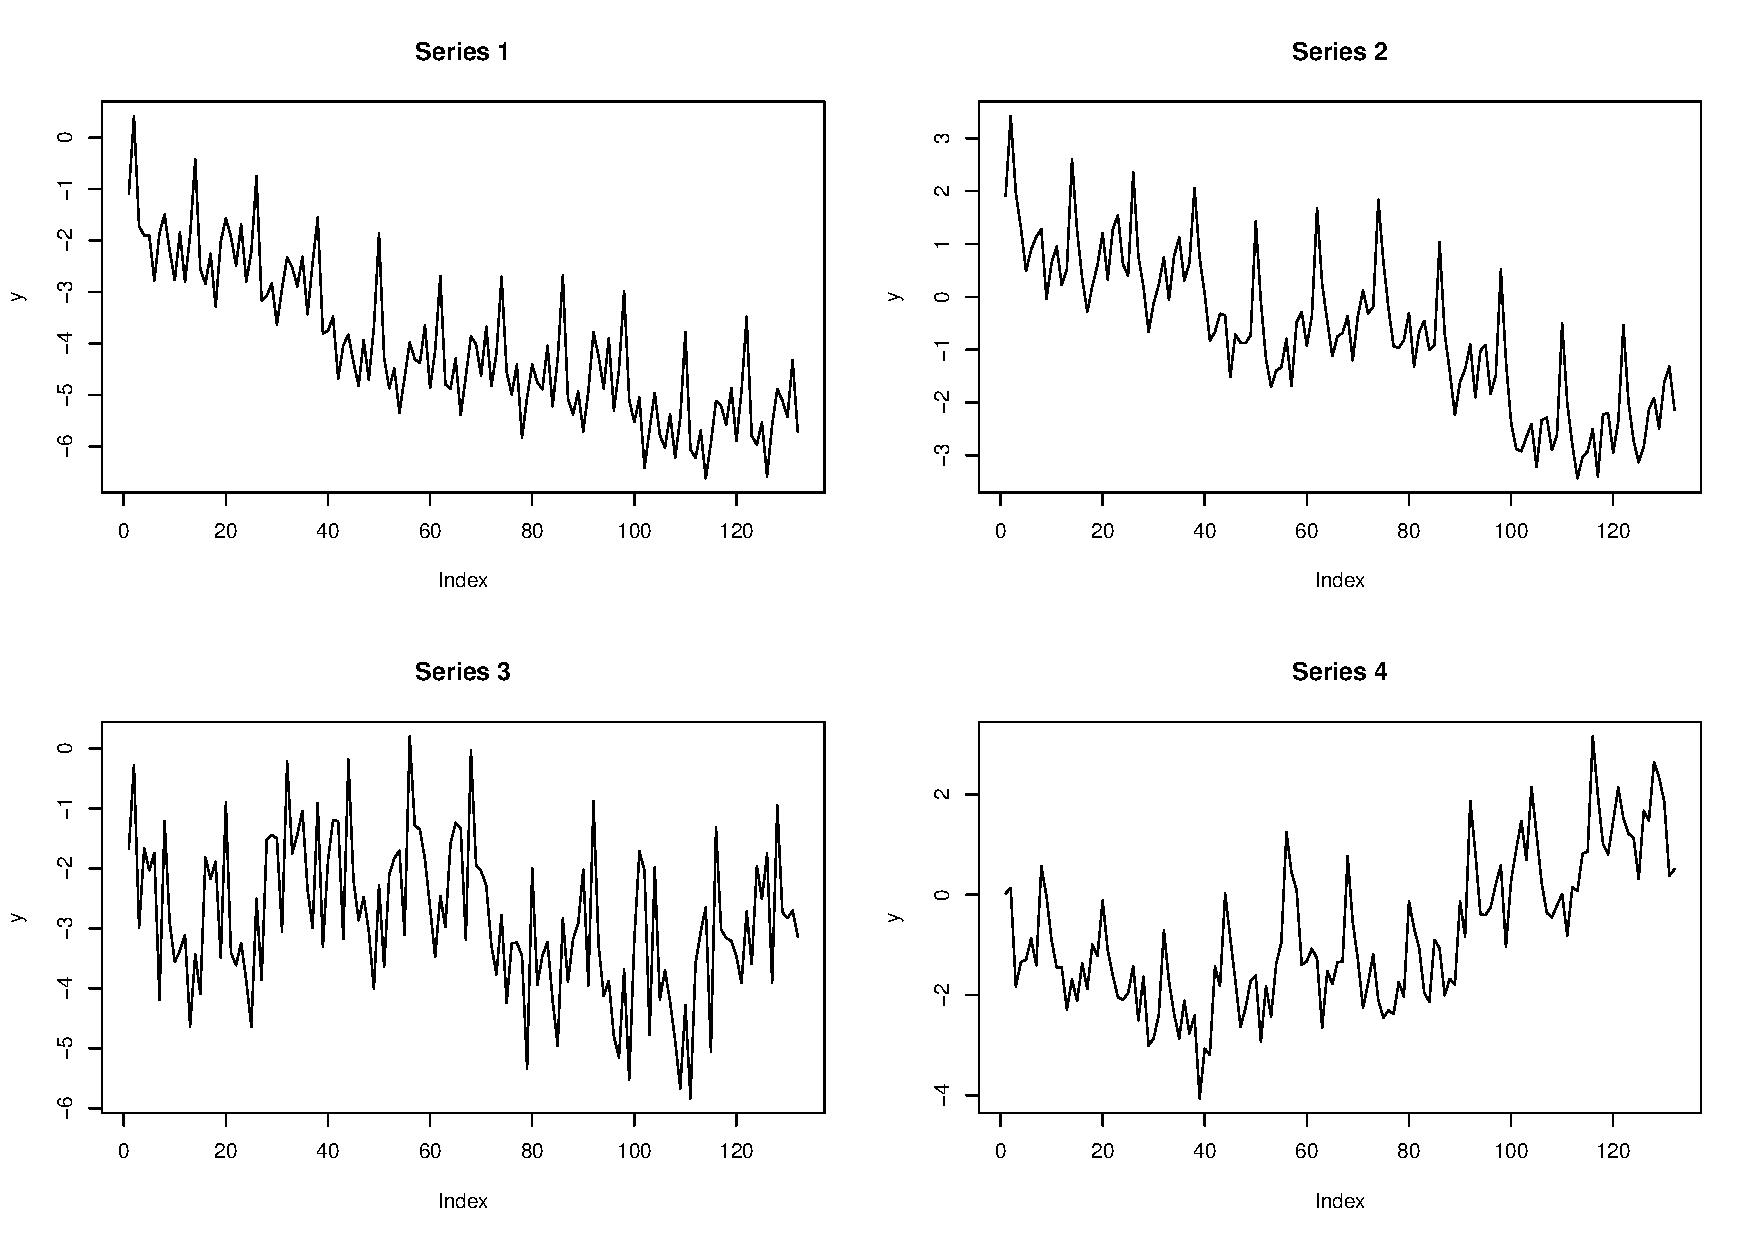
\includegraphics[width=\textwidth]{figures/sim1_example.pdf}
\caption{\label{fig:sim1_example} An example of simulated time series in Scenario 1.}
\end{figure}




\newpage

\bibliographystyle{agsm}
\bibliography{references.bib}
    
\end{document}